% !TeX spellcheck = en_US

\documentclass[t]{beamer}
\usetheme{Berlin}
\usecolortheme{beetle}
\useinnertheme[shadow]{rounded}
\useoutertheme{infolines}
\usepackage{amsmath}
\usepackage{bm}  %mogu pisati boldirane formule sa simbolima

%\usepackage{caption}
%\usepackage{subcaption}
\usepackage[utf8]{inputenc}
\setbeamersize{text margin left=3mm,text margin right=3mm}
\usepackage{subfig}
\usepackage{caption}
\usepackage{multicol} % multikolone
%\usepackage[figurename=Slika]{caption} % mijenja ime sa figure u slika
\usepackage{graphicx}
\graphicspath{{C:/Users/pc/Desktop/Thesis/keyword_extraction/paper/figures/}}

\setbeamertemplate{caption}[numbered]
\usepackage[plain]{algorithm2e}

\makeatother
\setbeamertemplate{headline}
{
	\leavevmode%
	\hbox{%
		\begin{beamercolorbox}[wd=1\paperwidth,ht=2.25ex,dp=1ex,center]{author in head/foot}%
			\usebeamerfont{author in head/foot}\insertshorttitle
		\end{beamercolorbox}%
	}
	\vskip0pt%
}


\makeatother
\setbeamertemplate{footline}
{
	\leavevmode%
	\hbox{%
		\begin{beamercolorbox}[wd=.2\paperwidth,ht=2.25ex,dp=1ex,center]{author in head/foot}%
			\usebeamerfont{author in head/foot}\insertshortauthor
		\end{beamercolorbox}%
		\begin{beamercolorbox}[wd=.4\paperwidth,ht=2.25ex,dp=1ex,center]{title in head/foot}%
			\usebeamerfont{title in head/foot}\insertshortinstitute
		\end{beamercolorbox}%
		\begin{beamercolorbox}[wd=.3\paperwidth,ht=2.25ex,dp=1ex,center]{title in head/foot}%
			\usebeamerfont{title in head/foot}\insertshortdate
		\end{beamercolorbox}%
		\begin{beamercolorbox}[wd=.1\paperwidth,ht=2.25ex,dp=1ex,center]{date in head/foot}%
			\insertframenumber{} / \inserttotalframenumber\hspace*{1ex}
	\end{beamercolorbox}}%
	\vskip0pt%
}


\makeatletter
\setbeamertemplate{navigation symbols}{}

\date{16. December 2023.}
\title[The title is quite quite quite quite quite quite long]{The title is quite quite quite quite quite quite long}
\author{Dinno Koluh}
\institute{Depratment of Computer Science and Engienering}



%Information to be included in the title page:

\title{Graph-Based Keyword Extraction fromScientific Paper Abstracts using Word Embeddings}
%c\date{Juni 2020. godine}

\settowidth{\leftmargini}{\usebeamertemplate{itemize item}}
\addtolength{\leftmargini}{\labelsep}

%\usepackage{beamerthemesplit}
%\usepackage{graphics}
\usepackage{float} % da slike nisu poremećene

\begin{document}
	
	
	\frame{
		\begin{center}
			{\scriptsize ALMA MATER STUDIORUM} \\
			{\scriptsize UNIVERSIT\`A  DI BOLOGNA} \\
			{\scriptsize DEPARTMENT OF COMPUTER SCIENCE AND ENGINEERING} \\
			{\scriptsize ARTIFICIAL INTELLIGENCE}\\[0.6cm]
			
			\hrule
			\vspace{0.1cm}
			{\Large Graph-Based Keyword Extraction from}\\[0.2cm]
			{\Large Scientific Paper Abstracts using Word Embeddings} \\
			\vspace{0.1cm}
			\hrule
			\vspace{0.20cm}
		\end{center}
		\hspace{1.5cm}    Author:       \hspace{4.8cm}          Supervisor:\\
		\hspace{1.0cm} Dinno Koluh  \hspace{3.7cm} Prof. Paolo Torroni\\
		\vspace{0.3cm}
		\hspace{7.6cm} Co-Supervisor\\
		\hspace{7cm} Dr. Federico Ruggeri\\
		\vspace{0.1cm}
		\begin{center}
			{ Bologna}\\
			{16. December 2023.}
		\end{center}	
	}
	
	
%	\begin{frame}
%		\frametitle{Sadržaj}
%		\tableofcontents
%	\end{frame}
	
	
	\begin{frame}{Problem statement}
		\begin{itemize}
			\item Problem of keyword extraction 
			\begin{itemize}
				\item Important words in text
				\item Inherently a ranking problem
			\end{itemize}
			\item Application to scientific paper abstracts
			\item Why model the problem as a graph?
			\begin{itemize}
				\item Well-established model
				\item Model text as a graph
				\item Ranking algorithms
			\end{itemize}
			\item The role of word embeddings
		\end{itemize}
	\end{frame}

	\begin{frame}{NLP Pipeline}
		\begin{itemize}
			\item Text preprocessing
			\item Broken down into blocks
			\begin{figure}[H]
				\centering
				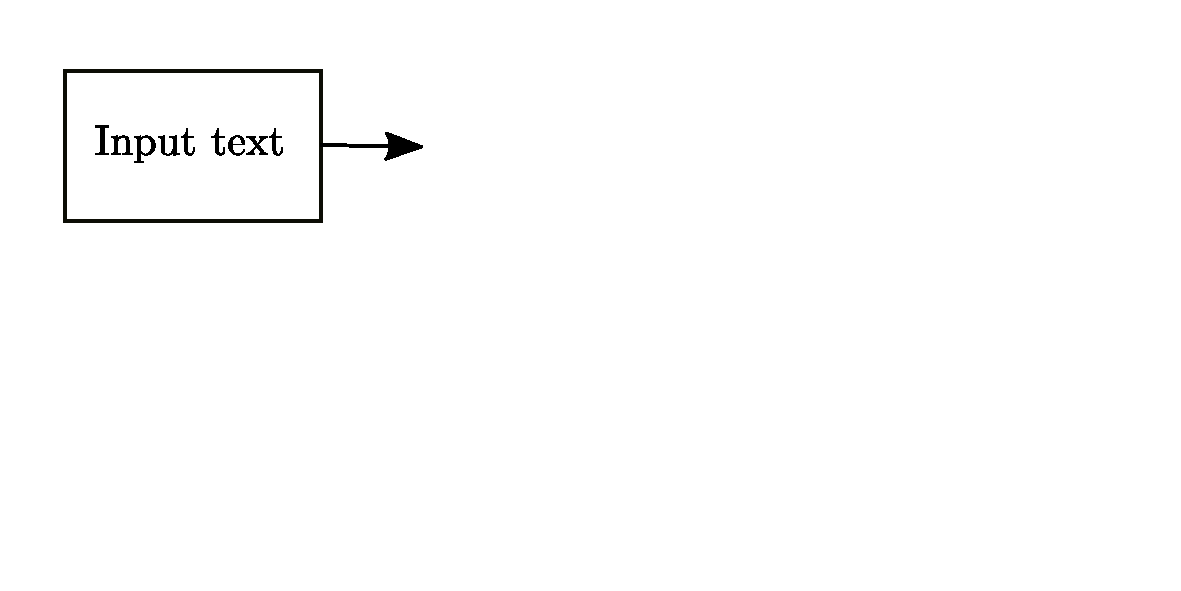
\includegraphics[scale=0.50]{NLP_pipeline}		
				%\captionsetup{justification=centering}
				\caption{The NLP pipeline}
				\label{NLP_pipeline_label}
			\end{figure}
		\end{itemize}
	\end{frame}

	\begin{frame}{Graph construction}
		\begin{itemize}

			%\item Co-occurrence matrix
			\begin{onlyenv}<1-1>
				\item Distributional hypothesis
				\begin{figure}[H]
					\hspace*{-0.5cm}
					\centering
					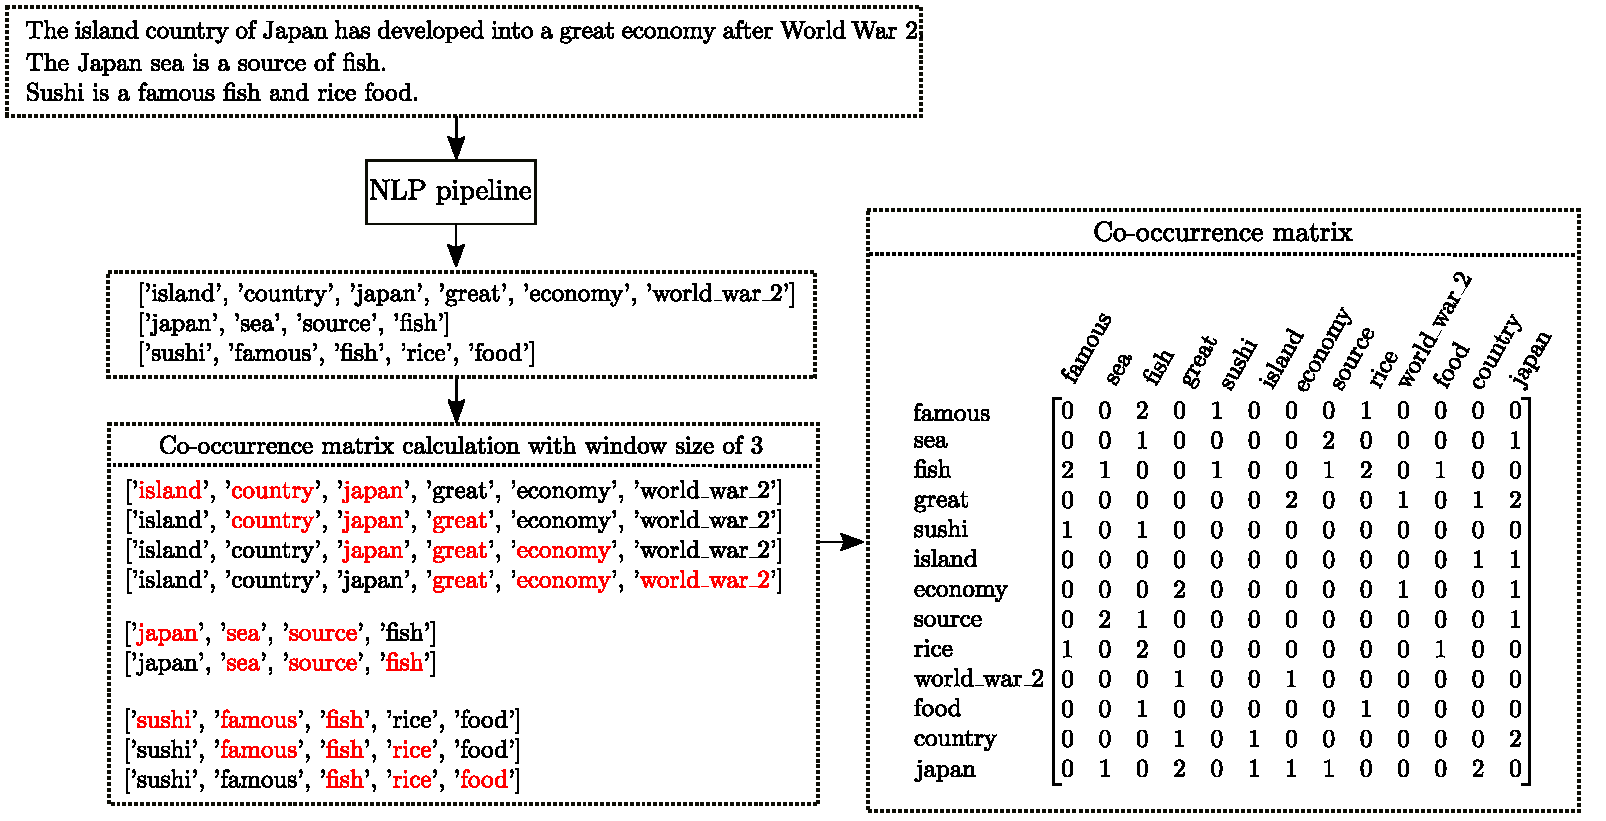
\includegraphics[scale=0.45]{context_diagram_horizontal}		
					%\captionsetup{justification=centering}
					\caption{Co-occurrence matrix construction}
					\label{context_diagram_horizontal}
				\end{figure}
			\end{onlyenv}
			
			\begin{onlyenv}<2-2>
				\begin{figure}[H]
					\vspace{-0.5cm}
					\hspace*{-0.5cm}
					\centering
					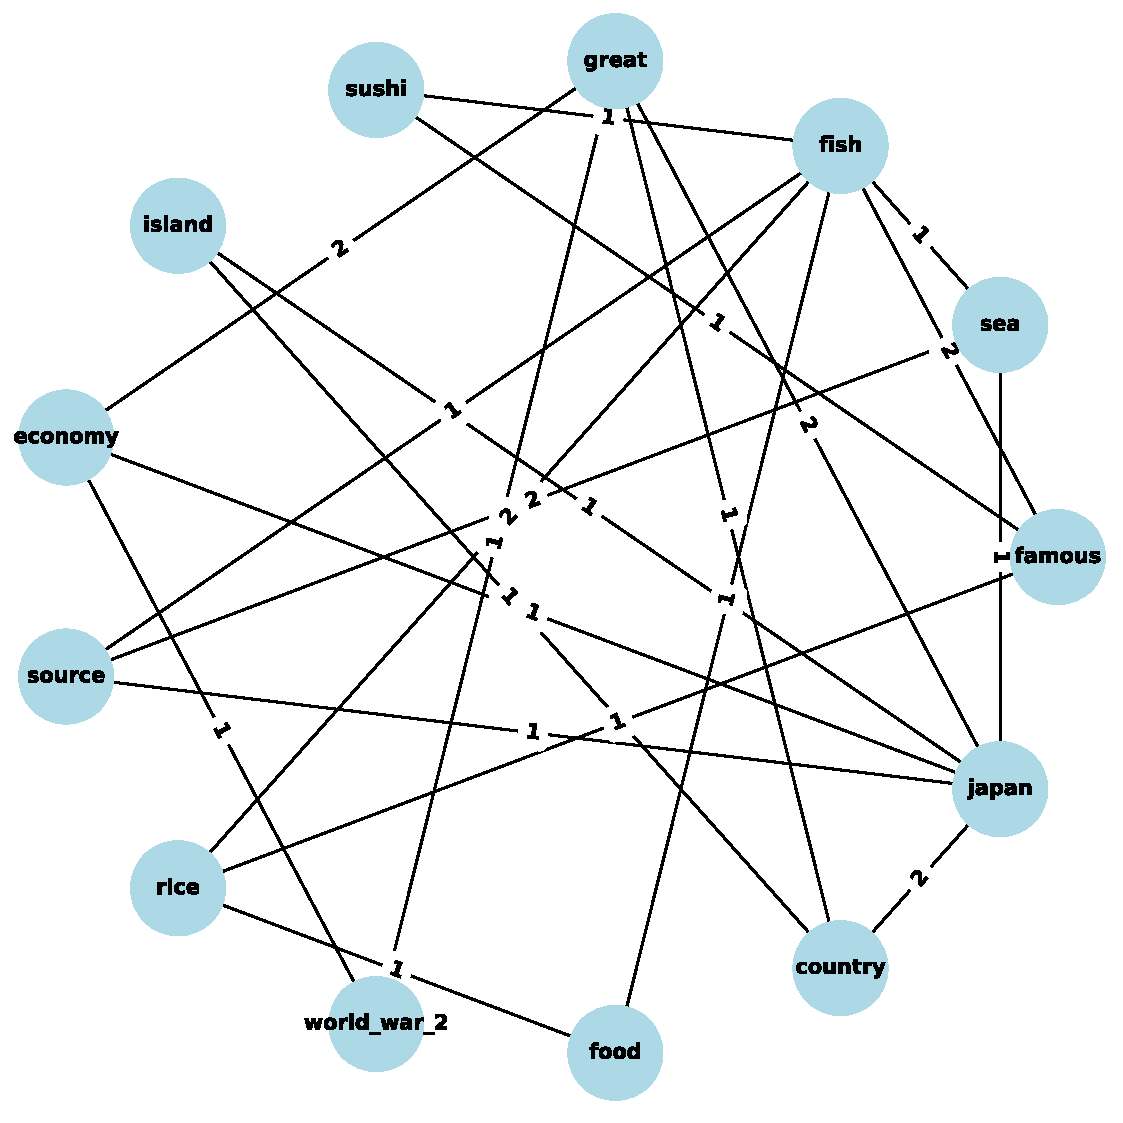
\includegraphics[scale=0.40]{graph_example}		
					%\captionsetup{justification=centering}
					\caption{Graph representation of the co-occurrence matrix}
					\label{}
				\end{figure}
			\end{onlyenv}
			
		\end{itemize}
	\end{frame}

	\begin{frame}{Ranking algorithms}
		\begin{itemize}
		\begin{onlyenv}<1-1>

				\item Degree centrality (based on node degree)
				\item Closeness centrality (based on distance to other nodes)
				\item Betweenness centrality (based on number of shortest paths that pass through the node i.e. information flow)
				\item Eigenvector centrality (based on direct and neighbour connections)
				\item PageRank algorithm (Google's web page ranking algorithm applied to text)
		\end{onlyenv}
	
		\begin{onlyenv}<2-2>
			\item Application on examples sentences:
			\item TABLE
		\end{onlyenv}

		\begin{onlyenv}<3-3>
			\item Full pipeline for keyword extraction
			\begin{figure}[H]
				\hspace*{-0.5cm}
				\centering
				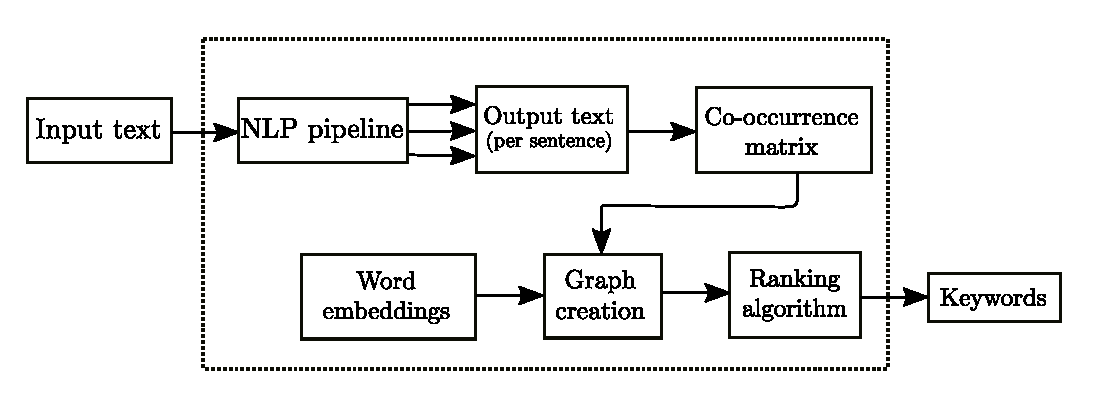
\includegraphics[scale=0.60]{full_pipeline}		
				%\captionsetup{justification=centering}
				\caption{Full pipeline of keyword extraction}
				\label{}
			\end{figure}
		\end{onlyenv}
		
		\end{itemize}
	\end{frame}


	\section{Experiments and Results}
	\begin{frame}{Experiments and Results}
		\begin{itemize}
			\begin{onlyenv}<1-1>
			\item Dataset: 5000 computer science paper abstracts with human assigned keywords, scraped from IEEE Xplore digital library
			\item Standard evaluation metrics (precision, recall, F-score)
			\item Important to address
			\begin{itemize}
				\item Human assigned keywords are subjective and can be generated
				\item Expected precision, recall and F-score from available literature in the range of $10 - 40 \%$
				\item Selecting the top \textit{n} keywords calculated by the model, where
				$ n $ is the number of true keywords from the dataset  
			\end{itemize}
			\end{onlyenv}
		
			\begin{onlyenv}<2-2>
				\item TABLE
			\end{onlyenv}
		\end{itemize}
	\end{frame}
	
%		\begin{itemize}
%	\item<1-> Težinska funkcija 
%	\begin{onlyenv}<1-3>
%		\begin{gather}\label{defineCostFunction}
%			f_c: \mathcal{C} \rightarrow \mathbb{R}_+ \\
%			f_c(\bm{q}) = c
%		\end{gather}
%	\end{onlyenv}
%	\item<2-> Težinska mapa
%	\item<3-> Kriteriji težinskih funkcija
%	
%\end{itemize}
	
	
	\begin{frame}
		\begin{center}
			\vspace{2cm}
			\Huge Q\&A
		\end{center}
	\end{frame}
	
	
\end{document}